% 图 5.1 几种磁有序/无序的自旋排列示意：(a) 铁磁 (b) 反铁磁 (c) 自旋玻璃 (d) 螺形 (e) 螺旋
\documentclass[tikz,border=5pt]{standalone}
\usetikzlibrary{arrows.meta,calc}
\usepackage{amsmath}
\usepackage{bm}
\usepackage{fontspec}
\setmainfont{Times New Roman}
\begin{document}
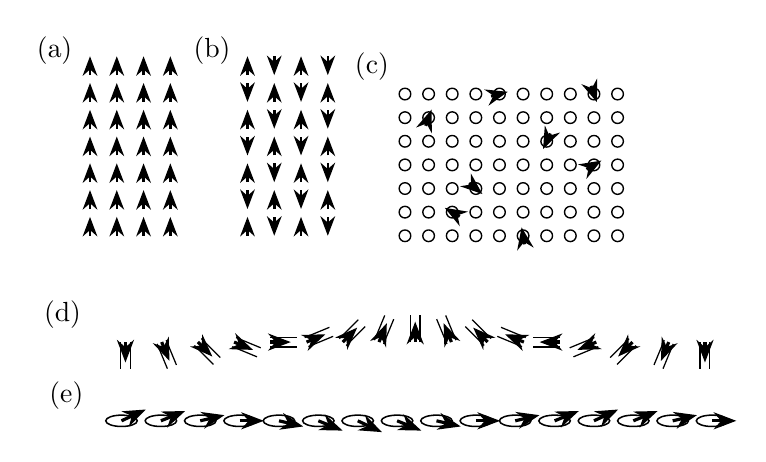
\begin{tikzpicture}[line width=0.8pt,>=Stealth]
% ---------- (a) ferromagnet: 4 cols x 7 rows, all up ----------
\begin{scope}[shift={(0,0)}]
\foreach \i in {0,...,3}{\foreach \j in {0,...,6}{
  \draw[->,line width=0.9] ({\i*0.34},{\j*0.34}) -- ({\i*0.34},{\j*0.34+0.24});}}
\node at (-0.45,2.35) {(a)};
\end{scope}
% ---------- (b) antiferromagnet: checkerboard ----------
\begin{scope}[shift={(2.0,0)}]
\foreach \i in {0,...,3}{\foreach \j in {0,...,6}{
  \pgfmathtruncatemacro{\s}{mod(\i+\j,2)}
  \ifnum\s=0
    \draw[->,line width=0.9] ({\i*0.34},{\j*0.34}) -- ({\i*0.34},{\j*0.34+0.24});
  \else
    \draw[<-,line width=0.9] ({\i*0.34},{\j*0.34}) -- ({\i*0.34},{\j*0.34+0.24});
  \fi}}
\node at (-0.45,2.35) {(b)};
\end{scope}
% ---------- (c) spin glass: 10x7 open circles, a few random arrows ----------
\begin{scope}[shift={(4.0,0)}]
\foreach \i in {0,...,9}{\foreach \j in {0,...,6}{
  \node[circle,draw,line width=0.5,inner sep=0,minimum size=4.2pt]
    at ({\i*0.30},{\j*0.30}) {};}}
% frozen moments (fixed pseudo-random set)
\foreach \i/\j/\a in {1/5/70, 3/2/-40, 4/6/15, 5/0/100, 6/4/-115, 8/3/30, 2/1/150, 8/6/-70}{
  \draw[->,line width=1.1] ({\i*0.30-0.11*cos(\a)},{\j*0.30-0.11*sin(\a)})
    -- ({\i*0.30+0.11*cos(\a)},{\j*0.30+0.11*sin(\a)});}
\node at (-0.42,2.15) {(c)};
\end{scope}
% ---------- (d) spiral: 17 in-plane darts, fixed step rotation ----------
\begin{scope}[shift={(0,-1.35)}]
\foreach \i in {0,...,16}{
  \pgfmathsetmacro{\a}{-90+\i*22.5}
  \pgfmathsetmacro{\cx}{0.45+\i*0.46}
  \draw[line width=0.45]
    ($(\cx,0)+(\a+90:0.062)$) -- ++(\a:0.34)
    ($(\cx,0)+(\a-90:0.062)$) -- ++(\a:0.34);
  \draw[->,line width=1.15] (\cx,0) -- ++(\a:0.26);}
\node at (-0.35,0.35) {(d)};
\end{scope}
% ---------- (e) helical: 16 side-view cones, precession about horizontal axis ----------
\begin{scope}[shift={(0,-2.35)}]
\foreach \i in {0,...,15}{
  \pgfmathsetmacro{\ph}{\i*30}
  \pgfmathsetmacro{\cx}{0.40+\i*0.50}
  \draw[line width=0.55] (\cx,0) ellipse [x radius=0.20, y radius=0.072];
  \draw[->,line width=1.15]
    (\cx,0) -- ++({0.34*cos(25)},{0.34*sin(25)*cos(\ph)});}
\node at (-0.30,0.32) {(e)};
\end{scope}
\end{tikzpicture}
\end{document}
